\paragraph{}
\begin{flushleft}
\textbf{Research Team}
\end{flushleft}

Klaus Sch�mann (Professor of Sociology), Paula Aleksandrowicz (Doctoral Fellow; until 06/2008), Stefan Baron (Doctoral Fellow; since 04/2007), Anette Fasang (Doctoral Fellow; until 08/2008; now Postdoctoral Fellow, Yale University), Sara-Izabella Geerdes (Doctoral Fellow), Daniel Schelkes (Doctoral Fellow; since 04/2008), Liuben Siarov (Doctoral Fellow BIGSSS; since 09/2008).

\paragraph{}
Socio-economic research on lifelong learning has to address the increasing impact of aging societies. We do this by applying a combination of economic research (e.g. human capital formation and accumulation) and sociological research (e.g. the social processes of inequality). Identifying market failures and understanding incentive structures with the potential to overcome unequal access to lifelong learning is part of our research program. The research group studies transitions over the life course and analyzes the impact of transitions on learning and employment careers. The life course perspective provides the central analytical tool that allows us to study individual trajectories, their institutional embeddedness, and the evolution of societies as a whole. 

\paragraph{}
Our research focuses on processes of social stratification as they are co-determined by learning processes for adults. We model social processes using two-step procedures: (1) we analyze participation in lifelong learning using age, cohort, and education levels as major determinants of participation and; (2) we observe that participation in lifelong learning is an important explanatory factor in processes of labor market mobility. In addition, our research group is carrying out projects with different firms as cooperation partners, focusing particularly on the aging of the workforce, health and safety at the workplace, strategies of lifelong learning, and skill needs assessment. We apply multilevel approaches that combine information from employees and management on the same topic, in a structured way. 

\paragraph{}
In each of these fields we analyze individual behavior as well as the impact of institutions on the life course. We have a particular interest in the link between working and learning as they concern individuals, households, firms and whole country systems. We study transitions throughout the life course that range from labor market entry and reentry after career breaks to gradual retirement; we pay special attention to changes in labor market institutions. These social dynamics are modeled using a transition theory that is based on notions of coupled oscillations (Sch�mann \& O'Connel, 2002) and synchronization techniques. In order to compare the impact of different institutional settings on individual behavior, we apply comparisons of industrial sectors, regions within a country, or US-EU-wide comparisons. Co-financed research projects deal with socioeconomic aspects of lifelong learning and institutional development in two major areas: (1) lifelong learning and the labor market, and (2) aging and the prevention of early retirement. \\


\begin{flushleft}
\textit{Central Reference } \\
\end{flushleft}


Sch�mann, Klaus (2002) "The theory of labour market transitions applied to the transitional labour market of education and training in: Klaus Sch�mann and Philip J. O'Connell (eds.), Education, Training and Employment Dynamics: Transitional Labour Markets in the European Union, Cheltenham, Edward Elgar, pp. 8-38.

\subsubsection{Lifelong Learning and the Labor Market}

\paragraph{}
\begin{flushleft}
\textbf{Research Program}
\end{flushleft}

Research in this area analyzes the link between lifelong learning and the labor market. We analyze sources of market failure, for example multiple factors responsible for underinvestment in lifelong learning. Persistent imbalances in supply and demand for training lead to a lack of participation in further training. Causal analyses of such behavior that seriously consider the evolution of the life course begin by investigating early labor market experiences and their implications for later experiences in the labor market. Analyses typically focus on transition processes like the first integration into the labor market, job to job transitions or further training transitions. 

\begin{figure}[htb]
  \begin{center}
    
\includegraphics[width=0.5\textwidth,height=10cm]{rr-Kfz-Mechaniker-bei-der-Arbeit.pdf}
  \end{center}
\end{figure}

\paragraph{}
\begin{flushleft}
\textbf{Research Highlights 2007/2008}
\end{flushleft}

Our analyses show that labor market integration of youth follows different trajectories depending on the young person's ethnic background. Young people with a second-generation migration background do not reach comparable entry-level labor market positions. In cases where they do reach jobs with similar types of contracts at entry, they nonetheless tend to have longer job search times (Geerdes et al. forthcoming, based on data from the Socio-economic Panel in Germany). Research also shows that youth and experienced workers do not compete for the same jobs in the labor market. Changes in economic growth have a much stronger impact on youth employment than they do on overall employment; this makes the youth labor market more volatile in general. This leads to better recruitment during favorable business cycles, but decreasing chances at times of slack growth (Hilbert et al., 2007)

\paragraph{}
Early labor market experiences, and particularly educational trajectories, are powerful predictors of participation in lifelong learning. Although the costs of training are due at the moment of participation, returns to training (e.g., increases in productivity or wages, job stability, or promotion) accrue only at some later point in time. Many employees therefore hesitate to take time out from productive work, or reduce working time in the labor market, in order to invest in further training. Risk aversion and budgetary constraints in the form of access to loans for purposes of learning also explain why people are reluctant to participate in training (Dissertation Siarov). In addition, firms might fear the "poaching" of training costs of employees by other firms (although this problem can be addressed by adequate contractual arrangements). Further ways of tackling the barriers to participation in training include: ensuring access to loans, promoting information availability, facilitating certification, the recognition of professional experience, and targeting groups that are the least likely to participate, such as less qualified and older employees. 

\paragraph{}
Research in these fields makes use of longitudinal data (both retrospective and panel), large European surveys, and our own data collected through our Lab III resources such as computer assisted telephone interviews, web-based surveys, or face-to-face interviews. Recent findings show that there are effective policies that can reduce stigmatization of older workers and combat the notion that older workers are less able or less willing to learn. It is therefore not sufficient to increase budgets; it is also necessary to tackle the stigma that perpetuates the view that older people are less interested in learning. Our results, based on an analysis of 20 years of household panel data from Germany, show that younger birth cohorts continue to have higher participation in further training than previous birth cohorts. The generation born between 1950 and 1960 participates on a higher level in further training than earlier cohorts (Sch�mann \& Baron, 2008). 

\paragraph{}
Participation in lifelong learning provides mutual benefits to individuals, firms and society as a whole, and innovative ways to co-finance lifelong learning are particularly promising policy solutions. However, participation in further training remains highly selective with respect to previously obtained levels of education. Our results from a comparative survey (the Eurobarometer, 2005) show that lower qualified individuals are indeed dissatisfied with their lower rates of participation in lifelong learning. This indicates that increasing targeted programs that match specific skill requirements should be successful at raising these low participation rates. 

\paragraph{}
We are also interested in discovering subjective and objective reasons for (non-) participation in lifelong learning (dissertation Baron). More specifically, with data from the interdisciplinary demopass project (see also 2.1) we examined potential influences on individuals' self-confidence in their own training competencies. Following social rational choice theories (e.g. Breen \& Goldthorpe, 1997, Esser, 2001), high self-confidence in one's own competencies is an important precondition for future participation in training. We found that people perceiving a higher training support by their supervisor and better learning climate tend to report a higher self-confidence (Baron \& Sch�mann, in prep.). This is particularly important for lower educated and older employees. It also constitutes new ways to enhance training participation rates of otherwise disadvantaged groups. However, we also identified mismatches between supervisors and associates in the evaluation of teams' training climate. Team members attach less importance to further training than their supervisors, whereas management does not meet employees' training needs.

\begin{figure}[htb]
  \begin{center}
    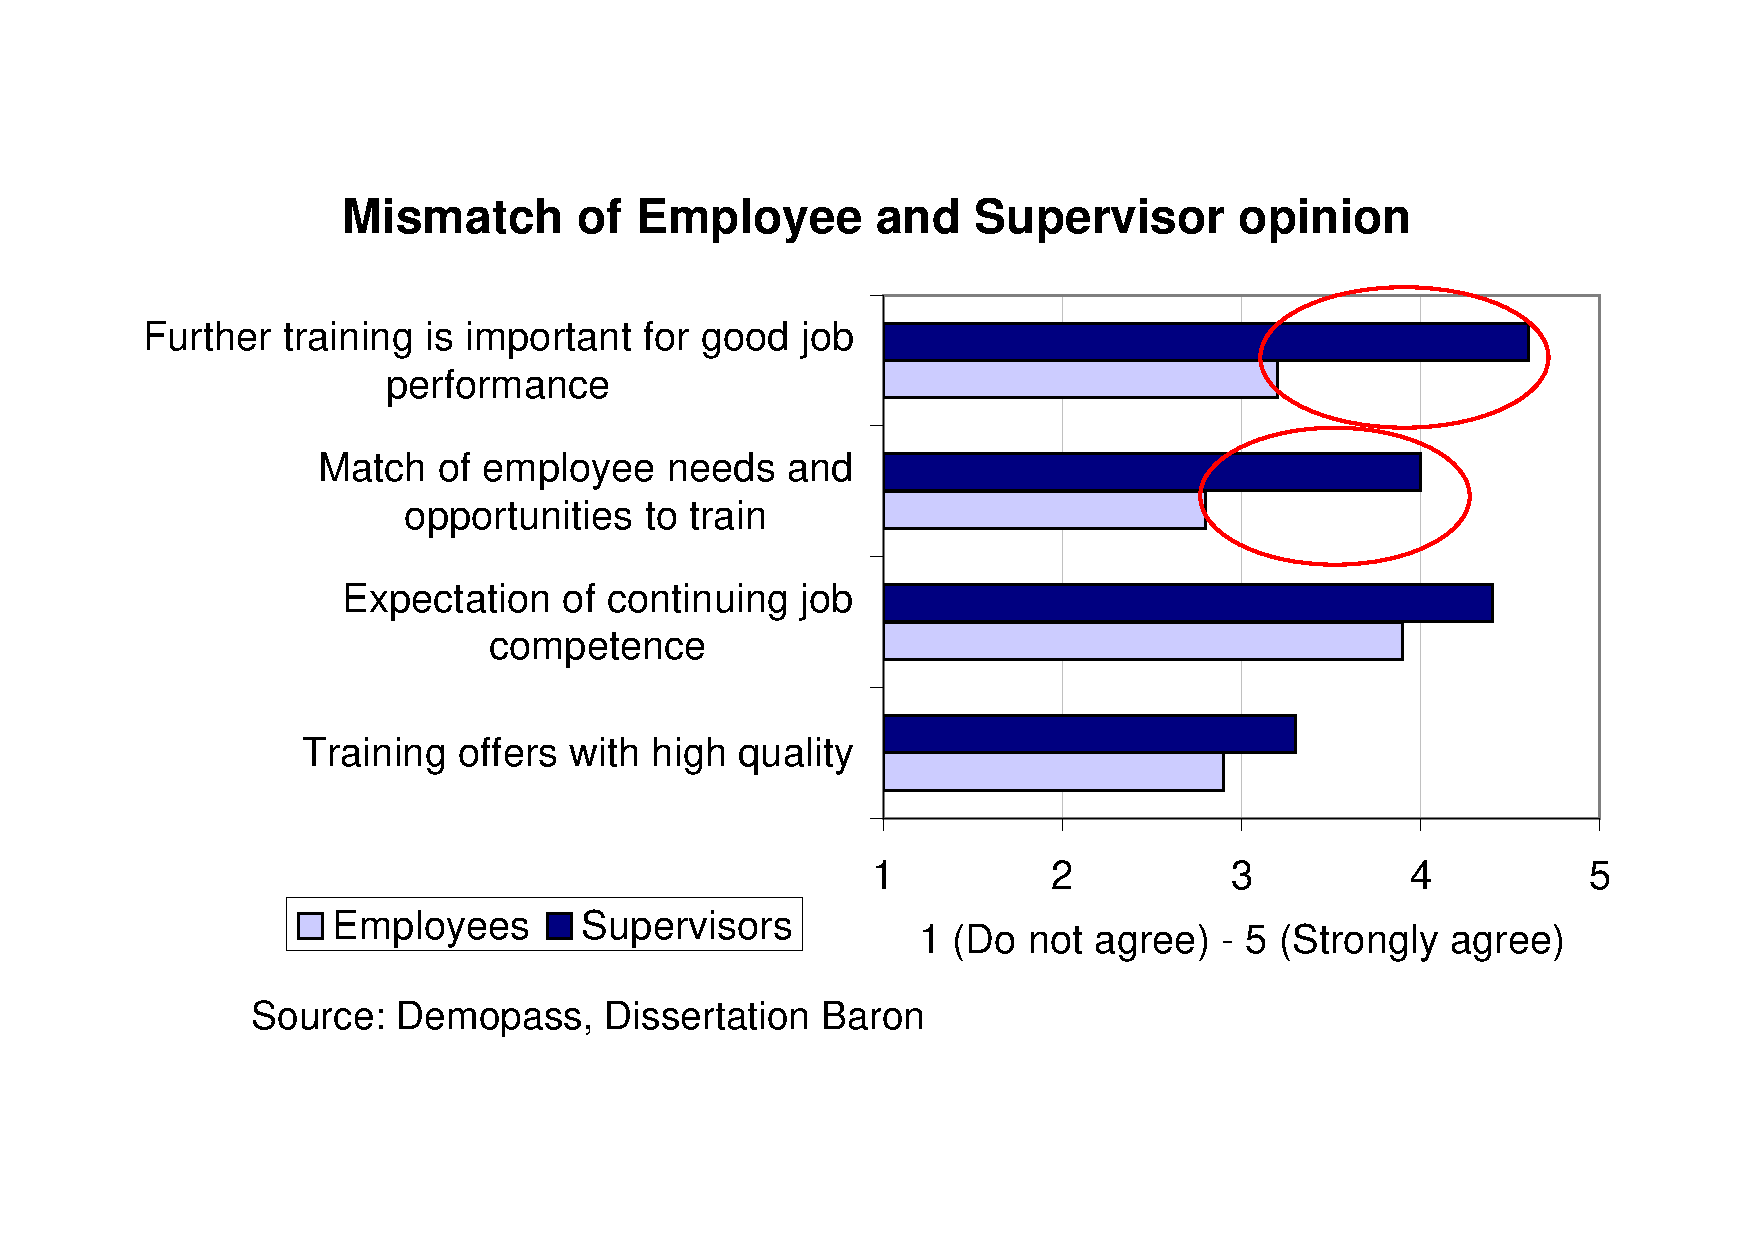
\includegraphics[width=0.5\textwidth,height=6.5cm]{MismatchFirmTrainingClimateChart.pdf}
    \caption{Matches/ Mismatches in firms' training climate. Source: Demopass, Dissertation Baron.}
  \end{center}
\end{figure}

\paragraph{}
Such mismatches can lead to discontent on both sides and as a direct consequence to lower participation rates in training. In sum, our results indicate that training programs should match specific skill requirements as closely as possible. This seems to be a necessary condition to raise the low participation rates of "silver" workers and low training groups in the labor market.

\subsubsection{Aging and the Prevention of Early Retirement}

\paragraph{}

\begin{flushleft}
\textbf{Research Program}
\end{flushleft}

The aging of the working population and the shrinking size of the population of working-age individuals in the near future will create a challenge to all components of welfare states. In order to enable a continuing potential for economic growth in rapidly aging societies, it will be necessary that more "silver workers" continue to work from each birth cohort. At the same time, new ways need to be found to facilitate an extension of working lives for these silver workers. This is the subject of our research interest in the field of productive aging. 

\begin{figure}[htb]
  \begin{center}
    
\includegraphics[width=0.4\textwidth,height=8cm]{rrgehorschutz.pdf}
  \end{center}
\end{figure}


\paragraph{}
\begin{flushleft}
\textbf{Research Highlights 2007/2008}
\end{flushleft}

We analyze this topic, for example, with emphasis on how to reverse the trend towards earlier and unequal retirement ages across industrially advanced societies. For this purpose we have compared retirement processes of the 1930-1940 birth cohorts in West Germany and those in the United Kingdom in order to assess how country specific labor market and pension regulations interact in structuring retirement processes. Our results indicate that, for Germany, the standardizing effects of the male breadwinner model occur across all different pathways to old-age pension. This has resulted in comparatively low household inequality at older ages. It is interesting to note that this somehow compensates for high personal inequality between women and men. For the United Kingdom, access to occupational or private pensions by at least one household member aggravates the divide between financially advantaged and less advantaged households (Fasang, 2008). 

\paragraph{}
In addition to labor and pension regulations, we include family biographies in our analyses of productive aging. We compare West Germany and the United Kingdom in order to assess how divorce effects the pension entrance of men and women born between 1930 and 1939. The life courses of these cohorts evolved in a strong male-breadwinner context in both countries, but were subject to different pension regulations (i.e. enforced pension sharing upon divorce in West Germany, and optional pension sharing in the United Kingdom). Pension sharing in Germany leads divorced women to enter old-age pension earlier and divorced men to enter later. In the United Kingdom, where pension sharing was not practiced, we find opposite effects (Fasang \& Sch�mann, 2008). 

\paragraph{}
Working jointly with local enterprises, we assessed the potential of older employees to continue working despite early retirement offers. The results of a company survey comparing early retirees and a similarly aged control group (still working) show that, while at work, employees have a high tendency to accept early retirement, but once in early retirement they soon begin to search for new challenges in the form of work or civic engagement (Aleksandrowicz et al., in press; see also 3.3). 

\paragraph{}
Overall, our work on retirement transitions and health and safety at work (Dissertation Schelkes) gives reason to believe that the prevention of early retirement is a multifaceted transition that requires careful analytical approaches in order to disentangle relevant causalities. The prevention of early retirement, and even the extension of working lives beyond 65, have become more feasible solutions based on sound analytical work. 

\paragraph{}
he recently approved project on "Job Mobility and Developmental Outcomes", co-financed by the Volkswagen Foundation (joint project with Staudinger and Godde; see also 2.2), allows us to assess the impact of cumulative labor market careers on individuals' learning strategies and adaptability at older ages. In a counterfactual design we will contrast matched (medium and low-skill) samples of persons with long labor market careers with meaningful, voluntary job changes, with those who have had few job changes. In a subsequent FMRI study both groups will participate in neurophysiologic tests. The results will give insights on cognitive and personality related adaptability (including learning strategies) of individuals in the two groups, and the interaction of adaptability with underlying neuronal processes. 

\subsubsection{Collaborations}

\begin{itemize}

\item Center for Research on Inequalities and the Life Course (CIQLE), Yale University; Prof. K.U. Mayer.
\item Center on Migration and Development, Princeton University; Prof. Marta Tienda.
\item Institute for Labour Studies (OSA), University of Tilburg; Prof. Ruud Muffels and Prof. Joop Schipers.  
\item Economic and Social Research Institute (ESRI), Dublin; Prof. Philip O'Connell.
\item Social Economic Research Rotterdam (SEOR), University of Rotterdam; Prof. Jaap de Koning. 
\item Institut f�r H�here Studien (IHS), Wien; Prof. Dr. Lorenz Lassnigg. 
\item MATISSE, Centre National de la Recherche Scientifique, Paris I; Prof. Bernard Gazier.
\item Centre for Labour Market Research (CARMA), Aalborg University; Prof. Per Madsen.
\item Research Centre for Education and the Labour Market (ROA), Maastricht University; Prof. Rolf van der Velden. 
\item Institute for Labour Studies (HIVA), Catholic University Leuven - co-ordinator Dr. Tom Vandenberghe.
\item University of North Carolina at Chapel Hill; Prof. Dr. Arne Kalleberg.

\end{itemize}

\subsubsection{Other Professional Activities}

\begin{itemize}
\item Consultant to OECD, European Commission DG Employment, Brussels and the European Foundation for the Improvement of Living and Working Conditions, Dublin.

\item{
\begin{flushleft}
\textit{Editorial Boards 2007/2008}
\end{flushleft}
Formation Emploi, Revue Fran�aise de Sciences Sociales (since 2000).}

\end{itemize} 

\subsubsection{Publications}

\begin{itemize}

\item Aleksandrowicz P., Fasang A., Sch�mann K., Staudinger U.M. (in press). Die Bedeutung der Arbeit beim vorzeitigen Ausscheiden aus dem Arbeitsleben, Zeitschrift f�r Gerontologie und Geriatrie. 

\item Sch�mann, K. \& Baron, S. (in press). Zustandsbeschreibung der Erwachsenenbildung in Deutschland und im europ�ischen Vergleich. In Staudinger, U. M. \& Heidemeier, H. (Hrsg.), Bildung und Lebenslanges Lernen als Chance und Herausforderung einer alternden Gesellschaft. Halle (Saale): Acta Nova Leopoldina. Stuttgart: Wissenschaftliche Verlagsgesellschaft.

\item ch�mann, K., \& Hilbert, C. (2008). Europe's Youth = Europe's Future. Benchmarking Working Europe (7), 43-49.

\item Sch�mann, K., Geerdes, S. \& Siarov, L. (2007). Institutional arrangements in support of adult competences and its nexus to flexicurity. In J�rgensen, Henning and Madsen, Per Kongsh�j (eds.), Flexicurity and Beyond: Finding a new agenda for the European Social Model�(pp. 421-450). Copenhagen : DJ�F Publishing.

\item Sch�mann K., Liuben, S. Geerdes, S. (2007). Lifelong Learning. Benchmarking Working Europe (6), 67-80. 

\item Fasang, A., Geerdes, S., Sch�mann, K., Siarov, L. 2007. Job satisfaction and labour market mobility. Report for the European Foundation for the Improvement of Living and Working Conditions: Dublin. http://www.eurofound.europa.eu/publications/htmlfiles/ef0710.htm Luxembourg: Office for Official Publications of the European Communities, ISBN 92-897-0955-3

\end{itemize}

